% Source: graduate-coursework/Sp26/CSCE763/Course_Assignments/HW1/HW1_CSCE_763_solutions.tex

\documentclass[border=4pt]{standalone}
\usepackage{amsmath}
\usepackage{amssymb}
\usepackage{graphicx}
\usepackage{tikz}
\usepackage{xcolor}
\usetikzlibrary{shapes.geometric, arrows.meta, positioning, patterns}

\definecolor{USC_Garnet}{HTML}{73000A}
\definecolor{USC_Sandstorm}{HTML}{FFF2E3}
\definecolor{USC_Black90}{HTML}{363636}
\definecolor{USC_Black70}{HTML}{5C5C5C}
\definecolor{USC_Black50}{HTML}{A2A2A2}
\definecolor{USC_Black10}{HTML}{ECECEC}
\definecolor{USC_Honeycomb}{HTML}{65780B}
\definecolor{USC_Atlantic}{HTML}{466A9F}
\definecolor{USC_Congaree}{HTML}{1F414D}
\definecolor{USC_Rose}{HTML}{CC2E40}
\definecolor{outputbg}{RGB}{245,245,245}

\begin{document}
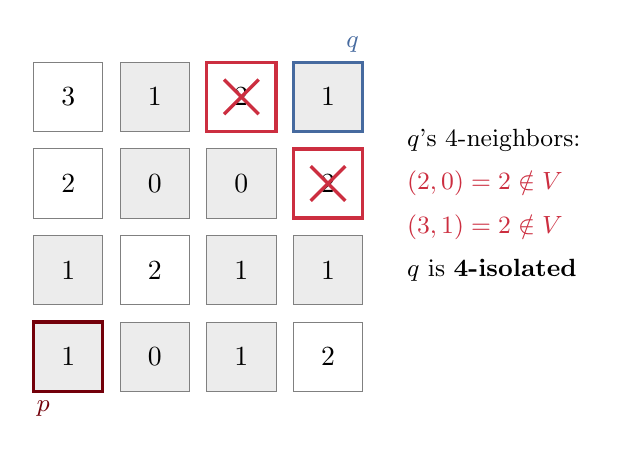
\begin{tikzpicture}[scale=1.1]
    % Shaded cells in V
    \fill[USC_Black10] (0.6,-0.4) rectangle (1.4,0.4);
    \fill[USC_Black10] (2.6,-0.4) rectangle (3.4,0.4);
    \fill[USC_Black10] (0.6,-1.4) rectangle (1.4,-0.6);
    \fill[USC_Black10] (1.6,-1.4) rectangle (2.4,-0.6);
    \fill[USC_Black10] (-0.4,-2.4) rectangle (0.4,-1.6);
    \fill[USC_Black10] (1.6,-2.4) rectangle (2.4,-1.6);
    \fill[USC_Black10] (2.6,-2.4) rectangle (3.4,-1.6);
    \fill[USC_Black10] (-0.4,-3.4) rectangle (0.4,-2.6);
    \fill[USC_Black10] (0.6,-3.4) rectangle (1.4,-2.6);
    \fill[USC_Black10] (1.6,-3.4) rectangle (2.4,-2.6);
    % Grid
    \draw[thin, gray] (-0.4,-0.4) rectangle (0.4,0.4); \node at (0,0) {3};
    \draw[thin, gray] (0.6,-0.4) rectangle (1.4,0.4); \node at (1,0) {1};
    \draw[thin, gray] (1.6,-0.4) rectangle (2.4,0.4); \node at (2,0) {2};
    \draw[thin, gray] (2.6,-0.4) rectangle (3.4,0.4); \node at (3,0) {1};
    \draw[thin, gray] (-0.4,-1.4) rectangle (0.4,-0.6); \node at (0,-1) {2};
    \draw[thin, gray] (0.6,-1.4) rectangle (1.4,-0.6); \node at (1,-1) {0};
    \draw[thin, gray] (1.6,-1.4) rectangle (2.4,-0.6); \node at (2,-1) {0};
    \draw[thin, gray] (2.6,-1.4) rectangle (3.4,-0.6); \node at (3,-1) {2};
    \draw[thin, gray] (-0.4,-2.4) rectangle (0.4,-1.6); \node at (0,-2) {1};
    \draw[thin, gray] (0.6,-2.4) rectangle (1.4,-1.6); \node at (1,-2) {2};
    \draw[thin, gray] (1.6,-2.4) rectangle (2.4,-1.6); \node at (2,-2) {1};
    \draw[thin, gray] (2.6,-2.4) rectangle (3.4,-1.6); \node at (3,-2) {1};
    \draw[thin, gray] (-0.4,-3.4) rectangle (0.4,-2.6); \node at (0,-3) {1};
    \draw[thin, gray] (0.6,-3.4) rectangle (1.4,-2.6); \node at (1,-3) {0};
    \draw[thin, gray] (1.6,-3.4) rectangle (2.4,-2.6); \node at (2,-3) {1};
    \draw[thin, gray] (2.6,-3.4) rectangle (3.4,-2.6); \node at (3,-3) {2};
    % Highlight q's 4-neighbors (all not in V)
    \draw[very thick, USC_Rose] (1.6,-0.4) rectangle (2.4,0.4);
    \draw[very thick, USC_Rose] (2.6,-1.4) rectangle (3.4,-0.6);
    % X marks on blocked neighbors
    \draw[USC_Rose, very thick] (1.8,-0.2) -- (2.2,0.2); \draw[USC_Rose, very thick] (1.8,0.2) -- (2.2,-0.2);
    \draw[USC_Rose, very thick] (2.8,-1.2) -- (3.2,-0.8); \draw[USC_Rose, very thick] (2.8,-0.8) -- (3.2,-1.2);
    % p and q
    \draw[very thick, USC_Garnet] (-0.4,-3.4) rectangle (0.4,-2.6);
    \draw[very thick, USC_Atlantic] (2.6,-0.4) rectangle (3.4,0.4);
    \node[below left, USC_Garnet, font=\bfseries\small] at (-0.1,-3.4) {$p$};
    \node[above right, USC_Atlantic, font=\bfseries\small] at (3.1,0.4) {$q$};
    % Label
    \node[right, font=\small] at (3.8,-0.5) {$q$'s 4-neighbors:};
    \node[right, font=\small, USC_Rose] at (3.8,-1.0) {$(2,0) = 2 \notin V$};
    \node[right, font=\small, USC_Rose] at (3.8,-1.5) {$(3,1) = 2 \notin V$};
    \node[right, font=\small] at (3.8,-2.0) {$q$ is \textbf{4-isolated}};
\end{tikzpicture}
\end{document}
